

\tikzset{every picture/.style={line width=0.75pt}} %set default line width to 0.75pt        

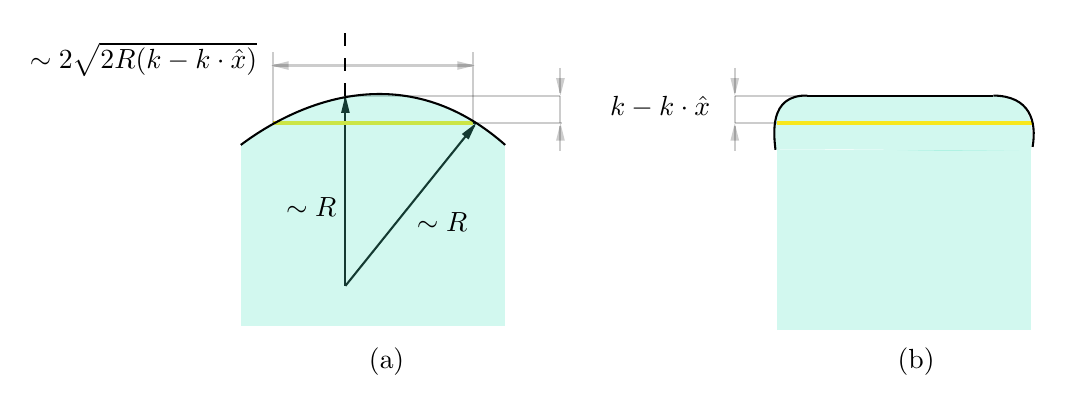
\begin{tikzpicture}[x=0.75pt,y=0.75pt,yscale=-0.7,xscale=0.7]
%uncomment if require: \path (0,300); %set diagram left start at 0, and has height of 300

%Straight Lines [id:da918640877893085] 
\draw [color={rgb, 255:red, 0; green, 0; blue, 0 }  ,draw opacity=0.2 ]   (485,113) -- (546,113) ;
%Shape: Polygon Curved [id:ds7664500750896397] 
\draw  [draw opacity=0][fill={rgb, 255:red, 80; green, 227; blue, 194 }  ,fill opacity=0.26 ] (525,95) .. controls (562,93.33) and (605,95.33) .. (663,94) .. controls (692,94.33) and (690,118.33) .. (689,131.33) .. controls (580,133.33) and (636,130.33) .. (513,131.33) .. controls (512,115.33) and (509,104.33) .. (525,95) -- cycle ;
%Straight Lines [id:da13905621281512137] 
\draw    (217,96) -- (217,225) ;
\draw [shift={(217,94)}, rotate = 90] [fill={rgb, 255:red, 0; green, 0; blue, 0 }  ][line width=0.08]  [draw opacity=0] (12,-3) -- (0,0) -- (12,3) -- cycle    ;
%Straight Lines [id:da5797227150605533] 
\draw    (305.75,114.56) -- (217,225) ;
\draw [shift={(307,113)}, rotate = 128.78] [fill={rgb, 255:red, 0; green, 0; blue, 0 }  ][line width=0.08]  [draw opacity=0] (12,-3) -- (0,0) -- (12,3) -- cycle    ;
%Straight Lines [id:da16317094389877962] 
\draw    (167,113) -- (307,113) ;
%Straight Lines [id:da11010905773487067] 
\draw  [dash pattern={on 4.5pt off 4.5pt}]  (217,94) -- (217,48) ;
%Straight Lines [id:da5866673345272755] 
\draw [color={rgb, 255:red, 248; green, 231; blue, 28 }  ,draw opacity=1 ][line width=1.5]    (167,113) -- (305,113) ;
%Straight Lines [id:da20682805869926613] 
\draw [color={rgb, 255:red, 0; green, 0; blue, 0 }  ,draw opacity=0.2 ]   (305,113) -- (366,113) ;
%Straight Lines [id:da5804485238189274] 
\draw [color={rgb, 255:red, 0; green, 0; blue, 0 }  ,draw opacity=0.2 ]   (217,94) -- (365,94) ;
%Straight Lines [id:da5258300587121219] 
\draw [color={rgb, 255:red, 0; green, 0; blue, 0 }  ,draw opacity=0.2 ]   (365,94) -- (365,113) ;
%Straight Lines [id:da0012951429125565017] 
\draw [color={rgb, 255:red, 0; green, 0; blue, 0 }  ,draw opacity=0.2 ]   (365,75) -- (365,92) ;
\draw [shift={(365,94)}, rotate = 270] [fill={rgb, 255:red, 0; green, 0; blue, 0 }  ,fill opacity=0.2 ][line width=0.08]  [draw opacity=0] (12,-3) -- (0,0) -- (12,3) -- cycle    ;
%Straight Lines [id:da4484021127908355] 
\draw [color={rgb, 255:red, 0; green, 0; blue, 0 }  ,draw opacity=0.2 ]   (365,115) -- (365,132) ;
\draw [shift={(365,113)}, rotate = 90] [fill={rgb, 255:red, 0; green, 0; blue, 0 }  ,fill opacity=0.2 ][line width=0.08]  [draw opacity=0] (12,-3) -- (0,0) -- (12,3) -- cycle    ;
%Straight Lines [id:da38084988502300243] 
\draw [color={rgb, 255:red, 0; green, 0; blue, 0 }  ,draw opacity=0.2 ]   (167,113) -- (167,64.33) ;
%Straight Lines [id:da3622174351254601] 
\draw [color={rgb, 255:red, 0; green, 0; blue, 0 }  ,draw opacity=0.2 ]   (305,113) -- (305,64.33) ;
%Straight Lines [id:da46269600902222074] 
\draw [color={rgb, 255:red, 0; green, 0; blue, 0 }  ,draw opacity=0.2 ][line width=0.75]    (168,73.33) -- (304,73.33) ;
\draw [shift={(306,73.33)}, rotate = 180] [fill={rgb, 255:red, 0; green, 0; blue, 0 }  ,fill opacity=0.2 ][line width=0.08]  [draw opacity=0] (12,-3) -- (0,0) -- (12,3) -- cycle    ;
\draw [shift={(166,73.33)}, rotate = 0] [fill={rgb, 255:red, 0; green, 0; blue, 0 }  ,fill opacity=0.2 ][line width=0.08]  [draw opacity=0] (12,-3) -- (0,0) -- (12,3) -- cycle    ;
%Shape: Rectangle [id:dp9029391185795892] 
\draw  [draw opacity=0][fill={rgb, 255:red, 80; green, 227; blue, 194 }  ,fill opacity=0.26 ] (145,128) -- (327,128) -- (327,252.33) -- (145,252.33) -- cycle ;
%Straight Lines [id:da7567604850412664] 
\draw    (535,94) -- (663,94) ;
%Straight Lines [id:da5213543435102419] 
\draw [color={rgb, 255:red, 0; green, 0; blue, 0 }  ,draw opacity=0.2 ]   (485,94) -- (546,94) ;
%Straight Lines [id:da4088065176465008] 
\draw [color={rgb, 255:red, 248; green, 231; blue, 28 }  ,draw opacity=1 ][line width=1.5]    (514,113) -- (690,113) ;
%Curve Lines [id:da11116595072683566] 
\draw [fill={rgb, 255:red, 80; green, 227; blue, 194 }  ,fill opacity=0.26 ]   (145,128) .. controls (185,98) and (258,67) .. (327,128) ;
%Curve Lines [id:da9329285452626859] 
\draw    (513,131.33) .. controls (512,121.33) and (508,93.33) .. (535,94) ;
%Curve Lines [id:da04442669114161091] 
\draw    (663,94) .. controls (688,94.33) and (693,111.33) .. (690,129.33) ;
%Shape: Rectangle [id:dp7639687953438465] 
\draw  [draw opacity=0][fill={rgb, 255:red, 80; green, 227; blue, 194 }  ,fill opacity=0.26 ] (514,131.33) -- (689,131.33) -- (689,255.67) -- (514,255.67) -- cycle ;
%Straight Lines [id:da07975102143157087] 
\draw [color={rgb, 255:red, 0; green, 0; blue, 0 }  ,draw opacity=0.2 ]   (485,94) -- (485,113) ;
%Straight Lines [id:da06258113523514597] 
\draw [color={rgb, 255:red, 0; green, 0; blue, 0 }  ,draw opacity=0.2 ]   (485,75) -- (485,92) ;
\draw [shift={(485,94)}, rotate = 270] [fill={rgb, 255:red, 0; green, 0; blue, 0 }  ,fill opacity=0.2 ][line width=0.08]  [draw opacity=0] (12,-3) -- (0,0) -- (12,3) -- cycle    ;
%Straight Lines [id:da7363046817146814] 
\draw [color={rgb, 255:red, 0; green, 0; blue, 0 }  ,draw opacity=0.2 ]   (485,115) -- (485,132) ;
\draw [shift={(485,113)}, rotate = 90] [fill={rgb, 255:red, 0; green, 0; blue, 0 }  ,fill opacity=0.2 ][line width=0.08]  [draw opacity=0] (12,-3) -- (0,0) -- (12,3) -- cycle    ;

% Text Node
\draw (174,162.4) node [anchor=north west][inner sep=0.75pt]    {$\sim R$};
% Text Node
\draw (397,92.4) node [anchor=north west][inner sep=0.75pt]    {$k-\boldsymbol{k} \cdot \hat{\boldsymbol{x}}$};
% Text Node
\draw (264,172.4) node [anchor=north west][inner sep=0.75pt]    {$\sim R$};
% Text Node
\draw (158.47,69.2) node [anchor=east] [inner sep=0.75pt]    {$\sim 2\sqrt{2R( k-\boldsymbol{k} \cdot \hat{\boldsymbol{x}})}$};
% Text Node
\draw (231,265.5) node [anchor=north west][inner sep=0.75pt]   [align=left] {(a)};
% Text Node
\draw (595,265.5) node [anchor=north west][inner sep=0.75pt]   [align=left] {(b)};


\end{tikzpicture}
